% https://tex.stackexchange.com/a/295021/173708
\documentclass[tikz,border=5]{standalone}
\usepackage{tikz}
\usetikzlibrary{calc}

\begin{document}
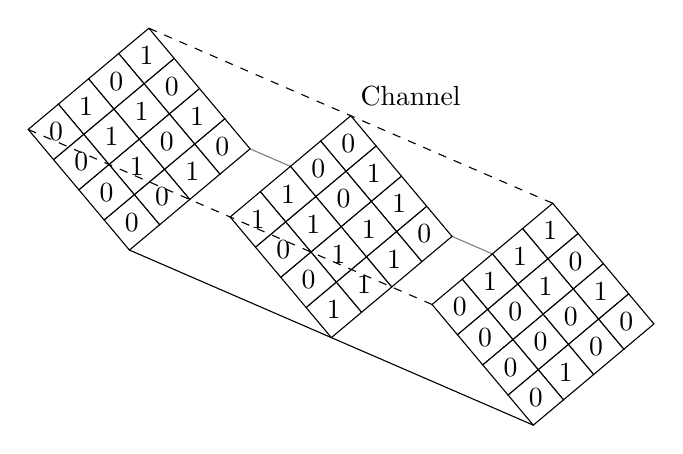
\begin{tikzpicture}[x=0.5cm,y=0.5cm]
    \begin{scope}[rotate=130,]
        \draw[gray] (-4  ,-1.5) -- (6  ,3.5);
    \end{scope}
    \foreach \shift in {-5,0,5}
    {
        \foreach \x in {1,...,4}
        {
            \foreach \y in {1,...,4}
            {
                \begin{scope}[rotate=130,shift={(\shift,0.5*\shift)},]
                    \draw[fill=white] (\x,\y) rectangle (\x+1,\y+1);
                    \node at (\x+0.5,\y+0.5) {\pgfmathrnd\pgfmathparse{round(\pgfmathresult)}
                        \pgfmathprintnumber[precision=1]{\pgfmathresult}};
                \end{scope}
            }
        }
    }
    \begin{scope}[rotate=130,]
        \draw         (-4, 2.5) -- (6  ,7.5);
        \draw[dashed] (0 , 2.5) -- (10,7.5);
        \draw[dashed] (0 ,-1.5) -- (10,3.5) node[midway,anchor=south west] {Channel};
    \end{scope}
\end{tikzpicture}
\end{document}